% \section{Model Architecture}
% \noindent In this section we will discuss about the architecture of base and target model.
% \begin{enumerate}
\section{Base Model} 

\noindent We have used GroundedSAM as a base or foundation model; GroundedSAM is a combination of GroundingDINO\cite{GroundingDINO} and Segment Anything Model\cite{Segment} to recognize and segment objects in an image with a given input text caption. 
% \begin{enumerate}
\subsection{Grounding DINO}
\noindent GroundingDINO is a zero-shot object detector. Most object identification models are developed to recognize a small set of predefined classes. The primary issue with this is that it needs to be more flexible. Whenever you wish to increase or modify the list of recognizable objects, you must gather data, label it, and retrain the model. Of course, doing this takes time and money. New object detection is made feasible without re-training a model thanks to zero-shot detectors like GroundinDINO. You must alter the prompt to get the model to recognize the objects you describe.

Grounding DINO combines the concepts published in the DINO\cite{dino} and GLIP papers\cite{glip}. DINO is an object detection method that is based on transformers. It gives state-of-the-art performance for object detection along with end-to-end optimization. At the same time, GLIP is more concerned with phrase grounding. This task tries to match phrases or words from a given text with equivalent visual elements in an image or video to connect textual descriptions to their corresponding visual representations.

It uses a text backbone like BERT to extract the text features and an Image backbone like Swin Transformer to extract Multiscale image features. Following the extraction of basic image and text features, the features are passed into the feature enhancer \ref{fig:DINO}, which contains several layers to combine features from several inputs. Different strategies are used to improve the text and image features.
A language-guided query selection module \ref{fig:DINO} is created to choose features more pertinent to the input text as decoder queries to exploit the input text for effectively guiding object detection. A cross-modality decoder is designed to merge the properties of text and visual modality properties. The model excels in numerous real-world tasks because it can recognize objects outside its training set and process language and visual content\cite{Ahmad_2023}.
\begin{figure}[h]
\centering
	\includegraphics*[width = 13cm]{images/DINO.png}
	 \caption{Grounding DINO overall Model}\cite{GroundingDINO}
	\label{fig:DINO}
\end{figure}
% \begin{center}
% 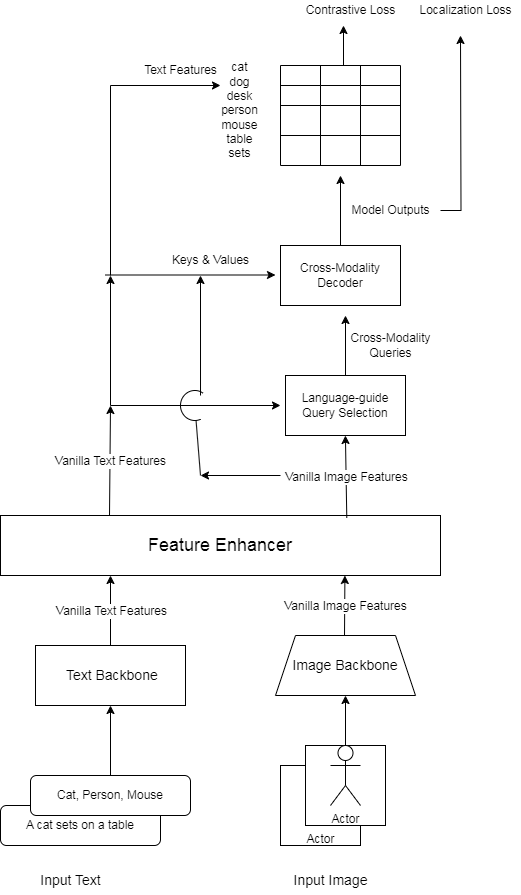
\includegraphics[width=13cm]{images/DINO.png}
% \end{center}

% \item Segment Anything Model:
\subsection{Segment Anything Model}

\noindent This model proposes a new dataset, model, and task for image segmentation.
The Segment Anything project builds a foundational or base model for image segmentation by using prompt engineering that solves various segmentation problems on new data.
% \begin{wrapfigure}{i}{}
%     \centering
%     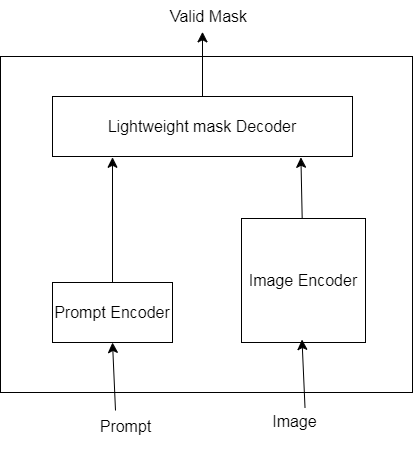
\includegraphics[width= 13cm]{images/segment.png}
%     \caption{Segment Anything Model}
%     \label{fig:segment}
% \end{wrapfigure}
% \begin{figure}[h]
% \centering
% 	\includegraphics*[width = 13cm]{images/segment.png}
% 	 \caption{Segment Anything Model}
% 	\label{fig:segment}
% \end{figure}

% \begin{center}
% 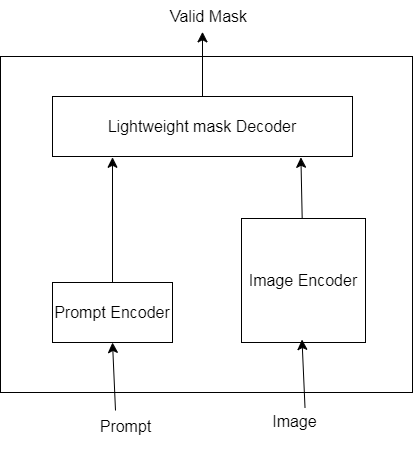
\includegraphics[width=8cm]{images/segment.png}
% \end{center}

The project's main elements are:
\begin{itemize}
    \item Task: A promptable segmentation task aims to return a valid segmentation mask for a given input prompt. Here valid means model should produce the most probable mask in the case of unclarity in the prompts provided. The segmentation prompt can be in the form of text, box, mask, or image.
    \item Model: The segment anything model consists of a lightweight mask decoder, image encoder, and prompt encoder \ref{fig:segment}. The mask decoder combines the information from the image encoder and prompt encoder to give a valid segmentation mask.

    \item Data: The required dataset is collected using a data engine. The Data Engine has three phases. SAM helps annotators generate the masks in the first stage. In the second stage, SAM automatically generates masks, and annotators concentrate on annotating the remaining objects. In the third stage, SAM is provided with a regular grid of points as input and generates the image masks.
\end{itemize}
The model's performance demonstrates that it can be a foundational model for image segmentation.
\begin{figure}[H]
\centering
	\includegraphics*[width = 7cm]{images/segment.png}
	 \caption{Segment Anything Model}\cite{Segment}
	\label{fig:segment}
\end{figure}
% \end{enumerate}

\section{Target Model} 

\noindent We are using YOLOv8 as a target model for surface floating object detection.

    \subsection{Characteristics}
    \noindent In YOLOv8, several features are to be prioritized. Object detection accuracy is increased by YOLOv8 compared to its predecessors by implementing new approaches and optimizations. It offers higher accuracy and faster inference speeds than existing object identification algorithms. It supports many backbones, including EfficientNet, ResNet, and CSPDarknet, allowing users to select the model suitable for their particular use case. Using adaptive training, YOLOv8 improves model performance by optimizing the learning rate and balancing the loss function during training. To increase the robustness and generalizability of the model, YOLOv8 uses sophisticated data augmentation techniques, including MixUp and CutMix. YOLOv8's architecture is adaptable, enabling users to quickly change the model's structure and parameters to meet their needs. It offers pre-trained models for convenient use and transfers learning across various datasets.

    \subsection{Architecture}
    
    \noindent The YOLOv8 architecture expands on earlier iterations of the YOLO algorithms. Because YOLO operates on the whole image simultaneously, it is rapid and effective. This is where the YOLOv8 differs from other object detection algorithms, which take a sliding window method that is expensive in computing. The convolutional neural network used by YOLOv8 comprises two primary sections the head and the backbone. The foundation of YOLOv8 is a modified version of the CSPDarknet53 architecture. Fifty-three convolutional layers make up this design, using cross-stage partial connections to enhance information transfer between the various layers. The head consists of many convolutional layers and fully linked layers. These layers are responsible for calculating bounding boxes, objectness scores, and class probabilities for the objects detected in an image. In Yolov8, bounding box predictions are made pixel-wise. An anchor-free detection head is introduced for this purpose. With the help of anchor-free detection \ref{fig:anchor}, an object detection model can predict the center of the object instead of the offset from the anchor box. The capability of YOLOv8 to carry out multi-scaled object identification is another crucial feature. The model uses a feature pyramid network to find items in an image with different sizes and scales.

\begin{figure}[H]
\centering
	\includegraphics*[width = 8cm]{images/Anchor-free.png}
	 \caption{Anchor Free Detection}
	\label{fig:anchor}
\end{figure}
% \begin{center}
% 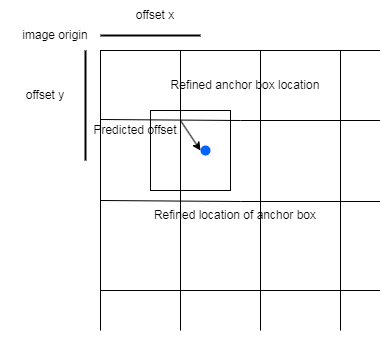
\includegraphics[width=10cm]{images/Anchor-free.png}
% \end{center}

\noindent Feature Pyramid Network (FPN)\cite{fpn} is a deep learning architecture designed to address the problem of object detection and recognition in images at multiple scales. In CNN architectures, the higher layers typically capture semantic information but lose spatial resolution, while lower layers capture finer spatial details but lack high-level semantics \ref{fig:variation}. FPN bridges this gap by constructing a multi-scale feature representation of the input image. FPN starts with a standard CNN for feature extraction from the input image. The backbone CNN processes the input image through several layers to obtain feature maps at different scales. These feature maps have decreasing spatial resolution but increasing semantic information as we move higher in the network \ref{fig:variation}.\\

\begin{figure}[H]
\centering
	\includegraphics*[width = 10cm]{images/variation.png}
	 \caption{Feature Extraction in FPN}
	\label{fig:variation}
\end{figure}
% \begin{center}
% 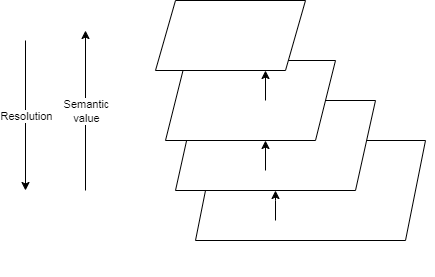
\includegraphics[width=10cm]{images/variation.png}
% \end{center}

\noindent FPN introduces a top-down pathway to upsample the feature maps and recover the lost spatial resolution. This is achieved by applying upsampling or interpolation on the higher-level feature maps. To combine the bottom-up and top-down pathways, FPN introduces lateral connections. These connections fuse the high-resolution features from the bottom-up pathway with the upsampled features from the top-down pathway \ref{fig:bottom}. The final output of FPN is a set of feature maps at multiple scales, each capturing different semantic and spatial information levels \ref{fig:bottom}.
\\\\

\begin{figure}[H]
\centering
	\includegraphics*[width = 12cm]{images/FPN.png}
	 \caption{Feature Pyramid Network}\cite{fpn}
	\label{fig:FPN}
\end{figure}
% \begin{center}
% 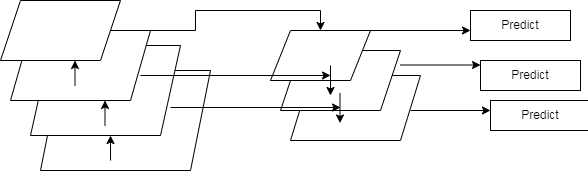
\includegraphics[width=12cm]{images/FPN.png}
% \end{center}

\begin{figure}[H]
\centering
	\includegraphics*[width = 13cm]{images/Bottom-up.png}
	 \caption{Bottom-up and Top-Down Pathway}\cite{fpn}
	\label{fig:bottom}
\end{figure}
% \begin{center}
% 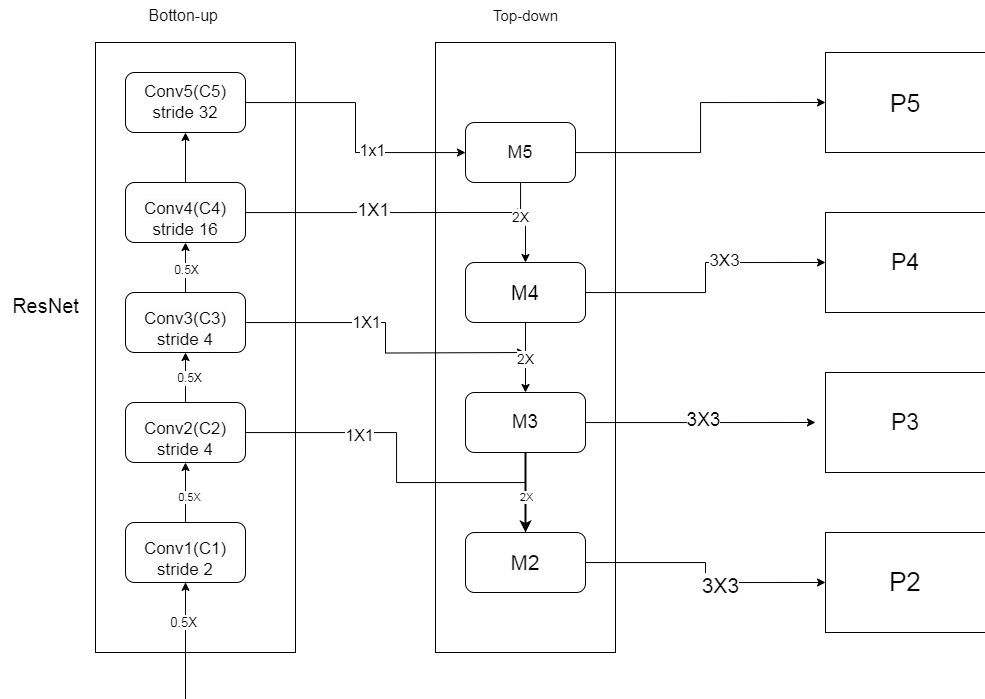
\includegraphics[width=12cm]{images/Bottom-up.png}
% \end{center}
% \end{enumerate}

\vspace{\baselineskip}

\noindent The use of FPN in object detection tasks has shown significant improvements in accuracy, especially when dealing with objects of different sizes within an image. By leveraging multiple-scale information, FPN enables the network to handle large and small objects better, improving object detection performance.


% \end{enumerate}
% \section{Thesis Objective}

%  \begin{enumerate}
%     \item To study and develop a solution for predicting the description of the images in real-time with good accuracy.
%     \item To further modify the existing models on image description generation with new modifications to reduce the complexity and training time of the proposed model.
%     \item To further automate the process of selecting the encoder for the neural network architecture to generate the description for the image.
%     \item To develop a native mobile application for fetching the description given in the image.
% \end{enumerate}
